% Második előadás
% FIXME: statikus vs dinamikus kezelés

\chapter{Függőségek}

\section{Bevezetés}
A függőségek gátolják a párhuzamos végrehajtást.

\section{Típusai}
\begin{itemize}
    \item adat
    \item vezérlés
    \item erősforrás
\end{itemize}

\section{Adat függőségek}
Probléma: az utasítás végrehajtáshoz egy előző utasítás eredményére van szükség.

\subsection{Csoportosítása}
\subsubsection{Jellege szerint}
\begin{itemize}
    \item utasítás szekvenciában (lineáris feldolgozás)
          \begin{itemize}
              \item valós függőség - nem teljesen megszüntethető (RAW - Read After Write)
                    \begin{itemize}
                        \item műveleti adatfüggőség
                        \item behívási adatfüggőség
                    \end{itemize}
              \item ál függőség - teljesen megszüntethető
                    \begin{itemize}
                        \item WAR - Write After Read
                        \item WAW - Write After Write
                    \end{itemize}
          \end{itemize}
    \item ciklusban
\end{itemize}
\subsubsection{Operandus típusa szerint}
\begin{itemize}
    \item regiszter
    \item memória
\end{itemize}

\subsection{Műveleti adatfüggőségek}
\paragraph{Probléma felvetés:} feltélezzük, hogy
\begin{itemize}
    \item a processzor 3 operandusos utasításokat használ
    \item 4 fokozatú futószalagos végrehajtás van (Fetch, Decode, Execute, WriteBack).
\end{itemize}
Ezekkel a feltételekkel két számot szeretnénk összeszorozni, az eredményt pedig megduplázni. Az utasításaink:
\begin{lstlisting}[language=Ant]
;I1
MUL r3,r2,1   ;r3 = r1 * r2
;I2
SHL r3        ;r3 * 2
\end{lstlisting}
Az utasítások végrehajtásának időbeli sorrendje:
\begin{center}
    \begin{tabular}{ c | c | c | c | c | c}
                           & t\textsubscript{1}   & t\textsubscript{2}      & t\textsubscript{3}   & t\textsubscript{4}    & t\textsubscript{5}    \\
        \hline
        I\textsubscript{1} & F\textsubscript{MUL} & D\textsubscript{r1, r2} & E\textsubscript{MUL} & W/B\textsubscript{r3} &                       \\
        \hline
        I\textsubscript{2} &                      & F\textsubscript{SHL}    & D\textsubscript{r3}  & E\textsubscript{SHL}  & W/B\textsubscript{r3}
    \end{tabular}
\end{center}
A probléma, hogy I\textsubscript{2} végrehajtása során, a dekódolási fázisban (t\textsubscript{3} időpillanat) szükség lenne az r3 regiszter értékére, viszont az csak t\textsubscript{4} időpillanatban áll elő (I\textsubscript{1} végrehajtásának writeback fázisában).
Tehát a futószalagos módszerrel párhuzamosított végrehajtás során műveleti adatfüggőség keletkezett, mivel az utasítások lehívása és végrehajtása között átfedés van.
Ilyenkor a műveletek elakadnak.
\paragraph{Megoldás:}egy speciális utasítás, a NOP (No Operand) használata az alábbi módon:
\begin{center}
    \begin{tabular}{ c | c | c | c | c | c | c | c}
                           & t\textsubscript{1}   & t\textsubscript{2}      & t\textsubscript{3}   & t\textsubscript{4}    & t\textsubscript{5}  & t\textsubscript{6}   & t\textsubscript{7}    \\
        \hline
        I\textsubscript{1} & F\textsubscript{MUL} & D\textsubscript{r1, r2} & E\textsubscript{MUL} & W/B\textsubscript{r3} &                     &                                              \\
        \hline
        I\textsubscript{2} &                      & F\textsubscript{SHL}    & NOP                  & NOP                   & D\textsubscript{r3} & E\textsubscript{SHL} & W/B\textsubscript{r3}
    \end{tabular}
\end{center}
\paragraph{Következmény:} a műveleteknek várakozniuk kell egymásra, két óraciklus késés keletkezik a futószalagon. Az ezeket követő utasításokhoz is be kell szúrni két NOP-ot, mivel a dekóder foglalt.
Ezt a jelenséget teljesen nem lehet megszüntetni, viszont a fékező hatást csökkenthetjük.
\paragraph{Kezelés:}operandus előrehozásával csökkenthető a fékező hatás, ez viszont extra hardvert igényel (hardveres, azaz dinamikus megoldás).
Extra hardver nélkül csak szoftveresen, azaz statikusan kezelhetjük a problémát.
Ilyenkor a compiler oldja meg a függőségek kezelését.
Általában előnyösebb a dinamikus megoldás.
\paragraph{Dinamikus megvalósítás:} az ALU-hoz tartozó rejtett regisztereket és az adatutakat a \ref{fig:operandus_elorehozas} ábra mutaja.
Alapesetben a MUL utasítás végrehajtása során az adat az r\textsubscript{1} és r\textsubscript{2} regiszterekből az src\textsubscript{1}, illetve src\textsubscript{2} regiszterekbe kerül, majd a művelet elvégzése után a rslt rejtett regiszteren keresztül visszaírásra kerül r\textsubscript{3}-ba.
Az adatút rövidítésének érdekében, extra hardver segítségével az rslt regiszter tartalmát közvetlenül visszavezethetjük az ALU egyik forrásregiszterébe. Ennek útja látható az ábrán pirossal.
Ekkor az utasítások végrehajtása az alábbi módon valósul meg:
\begin{center}
    \begin{tabular}{ c | c | c | c | c | c | c | c}
                           & t\textsubscript{1}   & t\textsubscript{2}      & t\textsubscript{3}   & t\textsubscript{4}    & t\textsubscript{5}    & t\textsubscript{6} & t\textsubscript{7} \\
        \hline
        I\textsubscript{1} & F\textsubscript{MUL} & D\textsubscript{r1, r2} & E\textsubscript{MUL} & W/B\textsubscript{r3} &                       &                                         \\
        \hline
        I\textsubscript{2} &                      & F\textsubscript{SHL}    & D                    & E\textsubscript{SHL}  & W/B\textsubscript{r3} &                    &
    \end{tabular}
\end{center}
Mivel már t\textsubscript{3} időpillanatban is rendelkezésre áll az SHL utasítás operandusa, két óraciklussal hamarabb kezdhető meg a művelet végrehajtása. Ezzel megszüntettük a késést.
Ezt a megoldást minden modern CPU használja.

\begin{figure}[H]
    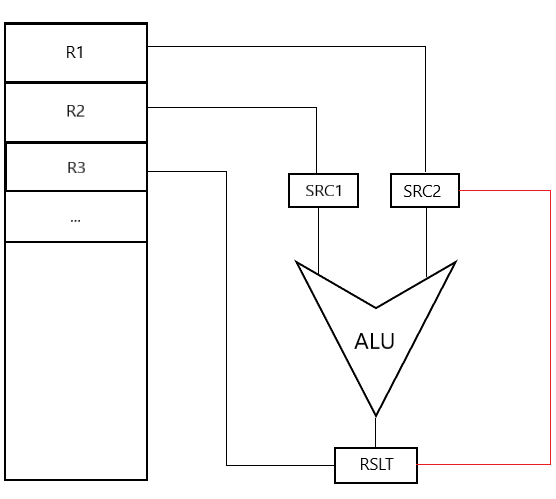
\includegraphics[width=0.6\textwidth]{operandus_elorehozas}
    \centering
    \caption{Az eredmény visszavezetése a forrás regiszterbe}
    \label{fig:operandus_elorehozas}
\end{figure}

\subsection{Lehívási adatfüggőség}
\paragraph{Probléma:} a regiszterekbe az operatív tárból (cache) töltjük be a szükséges adatokat, majd ezután a regiszterekből hívja le a végrehajtó egység (ALU).
A cache elérése viszont sok időt vesz igénybe.
Ennek látható az általános adatútja a \ref{fig:lehivas_elorehozas} ábrán, fekete vonallal jelölve.
\paragraph{Kezelés:} a folyamat gyorsítására extra hardvert alkalmazunk, amivel a cache-ből történő lehíváskor egyúttal a végrehajtó egységbe is betöltjük az adatot (piros vonal).
Így egy óraciklust megspórolhatunk.

\begin{figure}[H]
    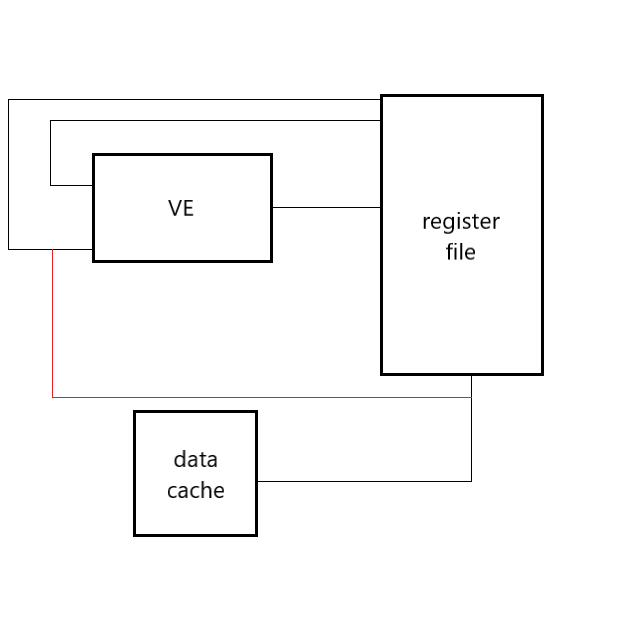
\includegraphics[width=0.6\textwidth]{lehivas_elorehozas}
    \centering
    \caption{A lehívott adat bevezetése a műveletvégző egységbe}
    \label{fig:lehivas_elorehozas}
\end{figure}

\subsection{WAR - Write After Read}

\paragraph{Probléma felvetés:} egy MUL utasítást egy ADD követ az alábbi módon:
\begin{lstlisting}[language=Ant]
    ;I1
    MUL r3,r2,1   ;r3 = r1 * r2
    ;I2
    ADD r2,r4,r5  ;r2 = r4 + r5
\end{lstlisting}
A szorzás (MUL) sokkal lassabb, mint az összeadás (ADD), ezért előfodulhat, hogy a párhuzamos
végrehajtás során I\textsubscript{2} hamarabb lefut, mint hogy I\textsubscript{1} betöltse a forrás operandust.
Mivel I\textsubscript{2} módosította I\textsubscript{1} bemeneti operandusát, a MUL utasítás hibás eredményt fog adni.
Következménye, hogy sérül a szekvenciális konzisztencia.
\paragraph{Megoldás:} r\textsubscript{2} tartalmát egy ideiglenes regiszterbe irányítjuk (pl. r\textsubscript{23}).
Ekkor az assmebly utasítások így néznek ki:
\begin{lstlisting}[language=Ant]
    ;I1
    MUL r3,r2,1   ;r3 = r1 * r2
    ;I2
    ADD r23,r4,r5 ;r23 = r4 + r5
\end{lstlisting}
Az r\textsubscript{23}$\,\to\,$r\textsubscript{2} hozzárendelést nyilvántartjuk, majd amikor a MUL utasítás végzett, visszaírjuk r\textsubscript{23} tartalmát r\textsubscript{2}-be.
Az átmeneti (átnevezési) regiszterek tulajdonságai:
\begin{itemize}
    \item új, önálló, de rejtett,
    \item saját címtartománnyal rendelkezik,
    \item a programozó számára traszparens,
    \item extra hardvernek számít.
\end{itemize}

\paragraph{Megjegyzés:} a regiszterkészletek csoportosítása:
\begin{itemize}
    \item architekturális: programozó használja,
    \item átnevezési: a vezérlés használja az álfüggőségek feloldására.
\end{itemize}

\subsection{WAW - Write After Write}
\paragraph{Probléma felvetés:} egy MUL utasítást egy ADD követ az alábbi módon:
\begin{lstlisting}[language=Ant]
    ;I1
    MUL r3,r2,1   ;r3 = r1 * r2
    ;I2
    ADD r3,r4,r5  ;r3 = r4 + r5
\end{lstlisting}
A szorzás (MUL) sokkal lassabb, mint az összeadás (ADD), ezért előfodulhat, hogy a párhuzamos
végrehajtás során I\textsubscript{1} később fut le, mint I\textsubscript{1}.
Mivel az eredményt ugyanabba a regiszterbe írják, ebben az esetben I\textsubscript{1} felülírja I\textsubscript{2} eredményét az r\textsubscript{3}-ban.
Ezzel sérül a szekvenciális konzisztencia.
\paragraph{Megoldás:} r\textsubscript{3} átirányítása egy átnevezési regiszterbe, az előbb leírt módon.

\subsection{Ciklusbeli függőség}

\paragraph{Probléma felvetés:}
egy ciklusban az előző iterációban kiszámolt adatot használunk fel, például:
\begin{algorithmic}
    \FOR{$i=2$ to $n$}
    \STATE X\textsubscript{i}$\leftarrow$A\textsubscript{i} * X\textsubscript{i-1} + B\textsubscript{i}
    \ENDFOR
\end{algorithmic}
\paragraph{Kezelés:} ez egy erős függőség, hardveresen nehezen feloldható. Megoldás az algoritmus áttervezése.

\section{Vezérlés függőségek}
Elágazások esetén léphetnek fel. Itt a statikus és dinamikus kezelésnek eltérő jelentése van, mint az adatfüggőségeknél. A statikus kezelés itt egy állandó, mindig alkalmazható eljárást jelent, míg a dinamikus kezelés az adott programtól függ.
\paragraph{Probléma felvetés:} az alábbi utasítássorozatban a feltétlen ugrás (JMP) egy SHL utasításra mutat:
\begin{lstlisting}[language=Ant]
    DIV
    MUL
    JMP ; SHL-re mutat
    ADD
    ...
    SHL
\end{lstlisting}
Ekkor a kritikus utasítások így követik egymást időben:
\begin{center}
    \begin{tabular}{ c | c | c | c | c | c | c }
            & t\textsubscript{1}   & t\textsubscript{2}   & t\textsubscript{3}   & t\textsubscript{4} & t\textsubscript{5} & t\textsubscript{6} \\
        \hline
        MUL & F\textsubscript{MUL} & D                    & E                    & W/B                &                    &                    \\
        \hline
        JMP &                      & F\textsubscript{JMP} & D                    & E                  & W/B                                     \\
        \hline
        ADD &                      &                      & F\textsubscript{ADD} & D                  & E                  & W/B
    \end{tabular}
\end{center}
A JMP utasítás az Execute fázisban állítja át a Program Countert, ezzel végzi el az ugrást.
A futószalag végrehajtás miatt azonban ekkorra már a következő utasítás, az ADD is lehívásra került, sőt, előfordulhat, hogy az azt követő utasítás is.
Ezek viszont fölösleges lépések. Ritkább esetekben a JMP-t követő utasítás be is fejeződhet, mire az ugrás végrehajtásra kerül, ami veszélyezteti az architekturális regisztertartalmakat.
\paragraph{Megoldás:} a probléma kezelése statikus, dinamikus, vagy spekulatív (branch prediction) módon történhet.
\paragraph{Kezelés utasítások átrendezésével (dinamikus):} compiler segítségével történő optimalizálás. A compiler megpróbálja átrendezni az utasítások sorrendjét.
Az előző kódrészlet optimalizált változata:
\begin{lstlisting}[language=Ant]
    JMP ; SHL-re mutat
    MUL
    DIV
    ADD
    ...
    SHL
\end{lstlisting}
Az optimalizálás utáni végrehajtási sorrend:
\begin{center}
    \begin{tabular}{ c | c | c | c | c | c | c | c }
            & t\textsubscript{1}   & t\textsubscript{2}   & t\textsubscript{3}   & t\textsubscript{4}   & t\textsubscript{5} & t\textsubscript{6} & t\textsubscript{7} \\
        \hline
        JMP & F\textsubscript{JMP} & D                    & E                    & W/B                  &                    &                                         \\
        \hline
        MUL &                      & F\textsubscript{MUL} & D                    & E                    & W/B                                                          \\
        \hline
        DIV &                      &                      & F\textsubscript{DIV} & D                    & E                  & W/B                                     \\
        \hline
        SHL &                      &                      &                      & F\textsubscript{SHL} & D                  & E                  & W/B
    \end{tabular}
\end{center}
A sorrend megváltoztatásával elértük, hogy amíg az ugrás végre nem hajtódik (t\textsubscript{3}), csak olyan utasításokat hívunk le, amiknek még az ugrás előtt kell lefutniuk.
Mire az ADD utasításhoz elérnénk, felülíródik a PC és a megfelelő utasítás hívódik le (SHL).
A módszer hátránya, hogy hatékonysága a futószalag fokozatok számának növelésével rohamosan csökken.
\paragraph{Kezelés NOP utasításokkal (statikus):} a JMP utasítás mögé egy vagy több NOP utasítás kerül be.
Ez a futószalag várakoztatását jelenti, amíg elő nem áll az ugráshoz szükséges PC. Ez az ún. ugrási buborék, nagysága $n-1$, ahol $n$ a futószalag fokozatok száma.
